As mentioned earlier, supersymmetry could solve the hierarchy problem and
provide a dark matter candidate, for this reason it has been the subject of
great experimental attention. Since the start of the \gls{lhc} the \gls{atlas}
and \gls{cms} experiments have performed a large number of searches for
\gls{susy} in many possible final states. \cref{fig:atlas_susy_summary}
illustrates the large number of searches performed by the \gls{atlas}
experiment, it can be seen in the first box that the squark and the gluino
production reaches the highest masses.

In the channel pursued in this thesis where two squarks are produced together
and decay directly to neutralinos, the 2-6 jets analysis excludes squarks up to
1.6~TeV. The $\squarkprod$ (compressed) search listed in
\cref{fig:atlas_susy_summary} is the one presented in
\cref{cha:monojet-signature} of this thesis. Other searches focus on third
generation squarks, the stop and sbottom where exclusions up to about 900~GeV
can be reached and on searches for production of \gls{susy} gauge bosons via the
electroweak interaction. In this situation the production cross sections are
much lower and the mass limits on these particles are generally below 1~TeV.
\begin{figure}[!htb]
  \centering
  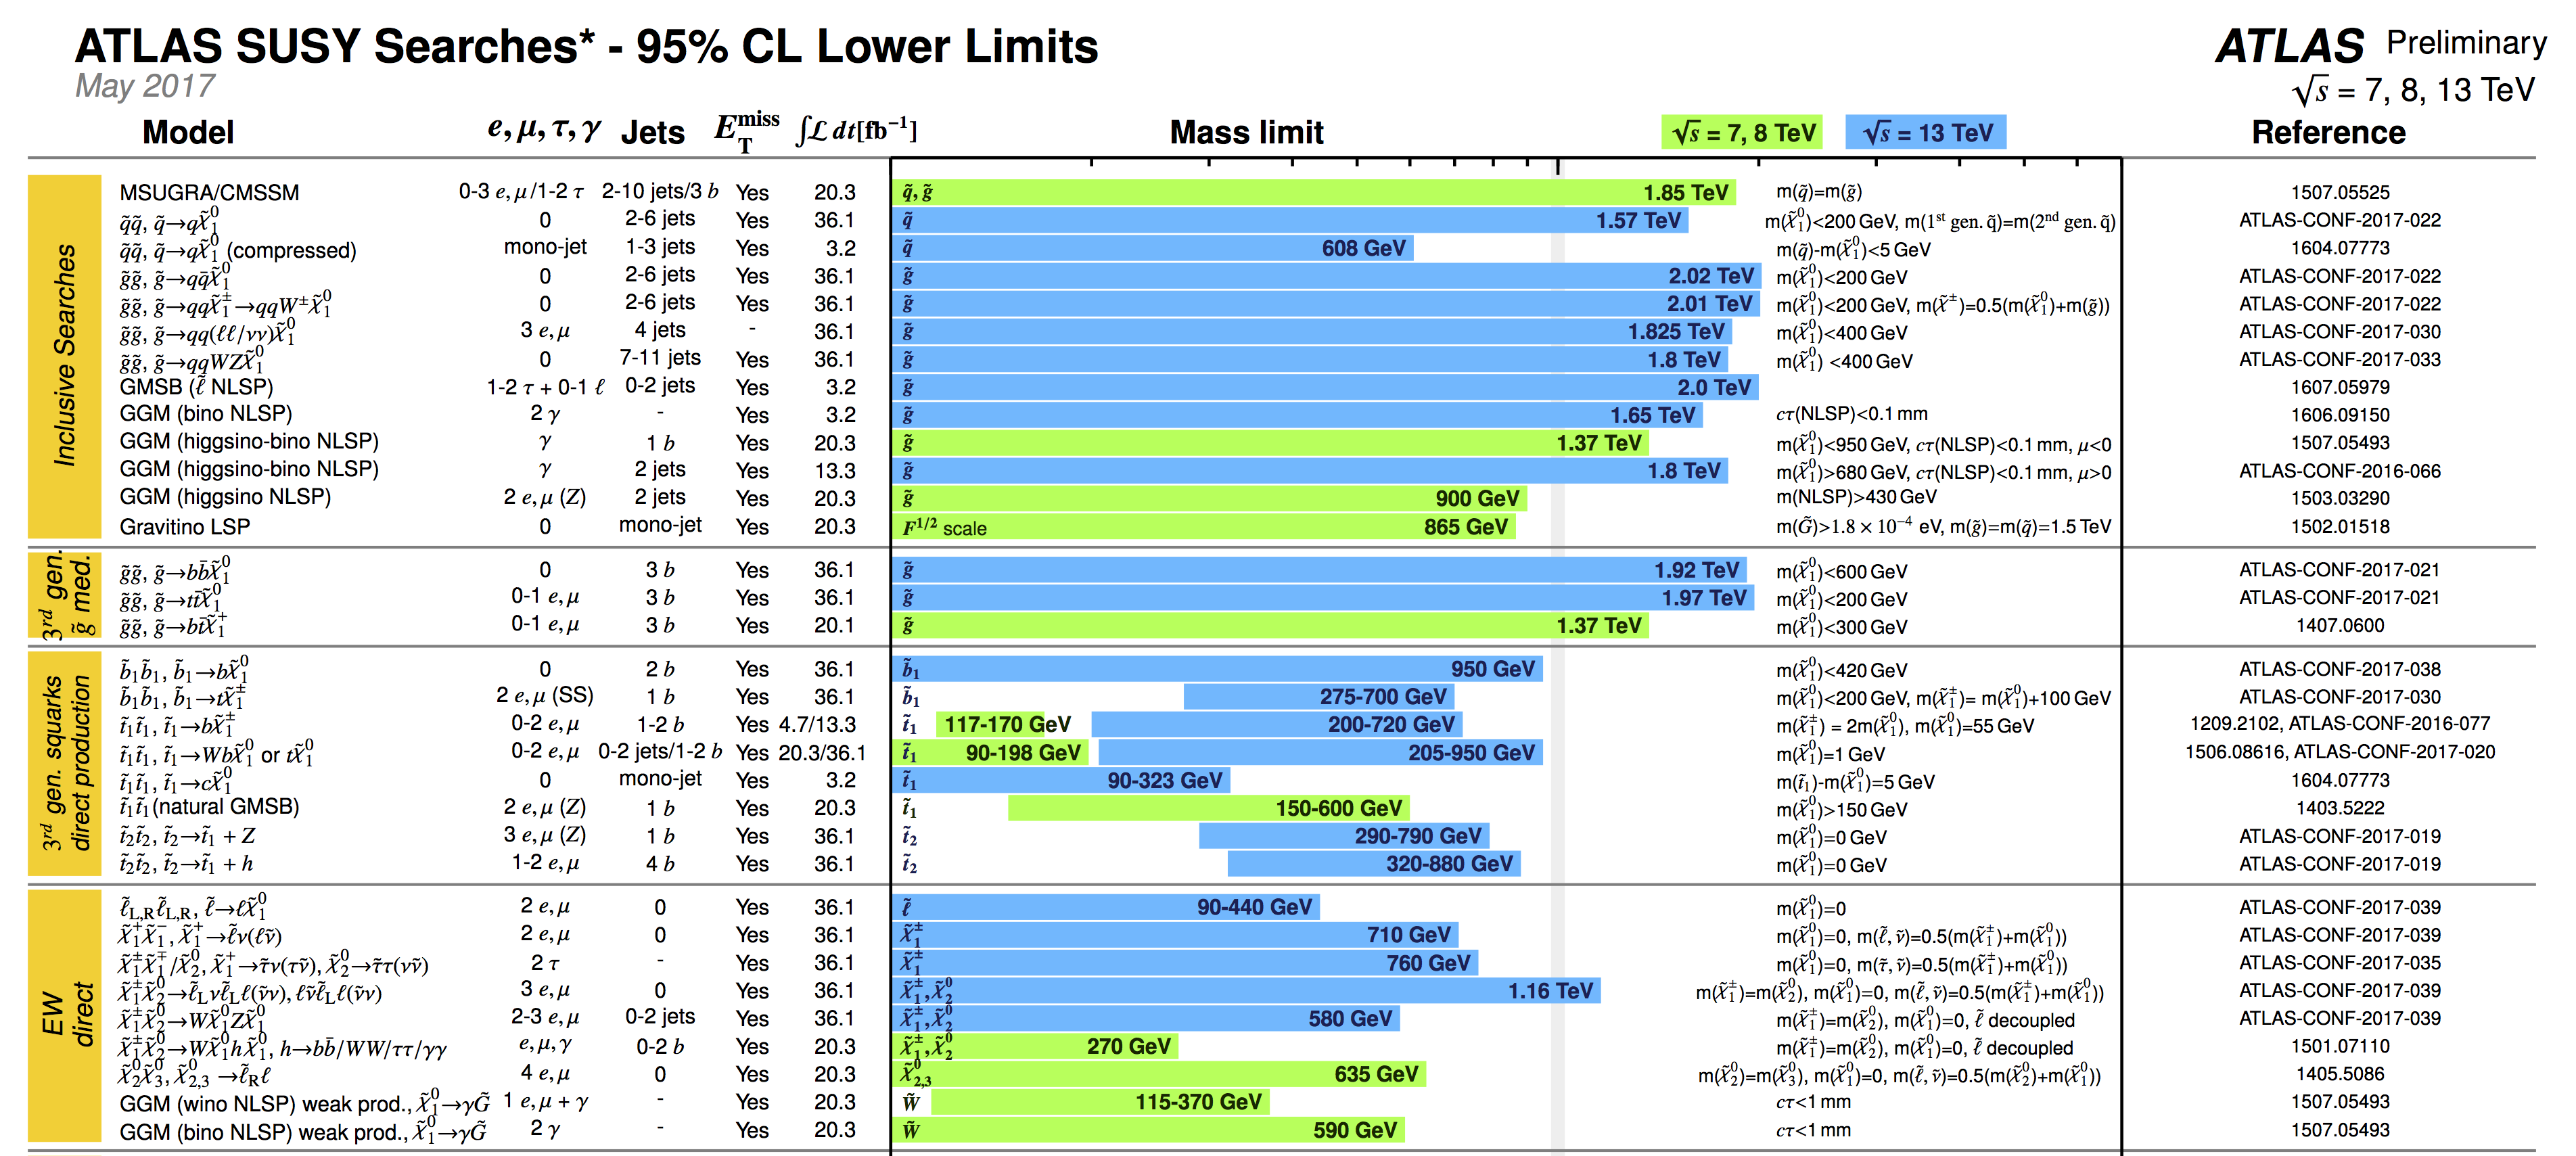
\includegraphics[width=.9\linewidth]{ATLAS_SUSY_summary}
  \caption{Representative selection of the mass reach in searches for
    supersymmetry with the \gls{atlas} detector~\cite{SUSYSummaryPlots}.}
  \label{fig:atlas_susy_summary}
\end{figure}
%%% Local Variables:
%%% mode: latex
%%% TeX-master: "../search_for_DM_LED_with_ATLAS"
%%% End:
